\chapter{Zadania dodatkowe}
	\label{ch:dod}
	\section{PID}
		\label{sec:PID}
		Algorytm PID oblicze przyszłe sterowanie na podstawie wartości, pochodnej i całki uchybu w odpowiednich proporcjach. Popularną sposobem strojenia tego regulatora jest metoda Zieglera-Nicholsa, która polega na doprowadzenie obiektu na granice stabilności przy wyłączonych członach I oraz D, zmierzenia okresu drgań a następnie podstawieniu odpowiednich wartości do wzoru. W przypadku obiektu z zadania obiekt był na granicy stabilności (w we wszystkich zadanych przez nas punktach pracy) przy $K_p=4$, co można zaobserwować na rys. \ref{fig:PID0}.
		
		\begin{figure}[h!]
			\centering
			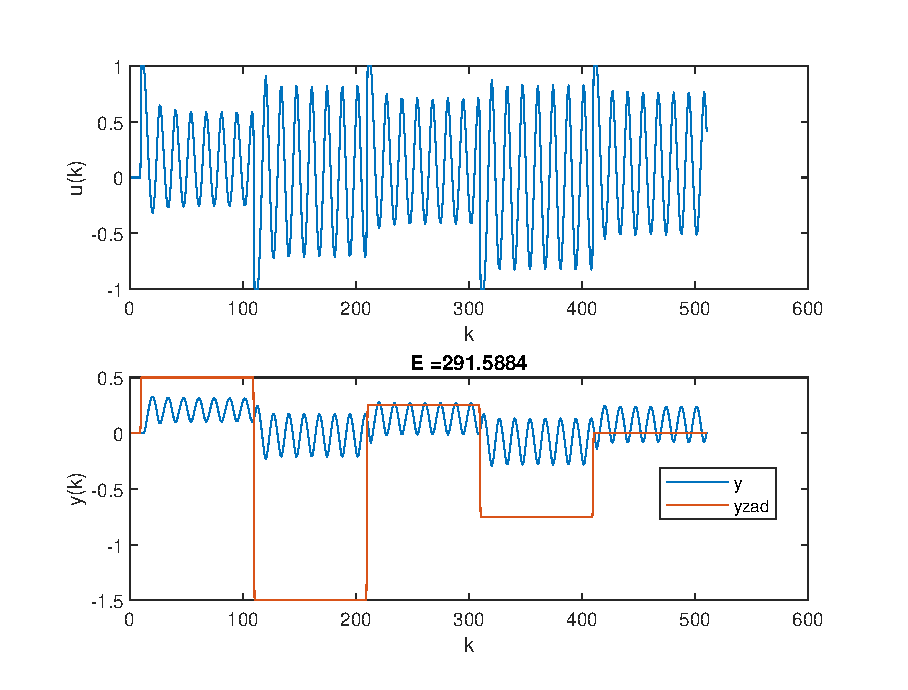
\includegraphics[width=\linewidth]{img/strojeniePID_Kp_4_Ti_duzo_Td_0.eps}
			\caption{Działanie regulatora PID z nastawami Kp = 4, Ti = Inf, Td = 0}
			\label{fig:PID0}
		\end{figure}
		
		\newpage
		Następnie, po podstawieniu zmierzonych wartości (okres drgań $T_u=13$) otrzymaliśmy przebieg przedstawiony na rys. \ref{fig:PID1}.
		Widać, że regulator próbuje naśladować przebieg wartości zadanej, i robi to nie najgorzej (mimo bardzo ostrego sterowania), lecz dla niektórych punktów pracy pojawiają się niegasnące oscylacje. Nastrojony w ten sposób regulator wydaje się dobrze radzić sobie w bliskości granicy przedziału sterowania, a gorzej będąc w jego centrum.
		
		\begin{figure}[h!]
			\centering
			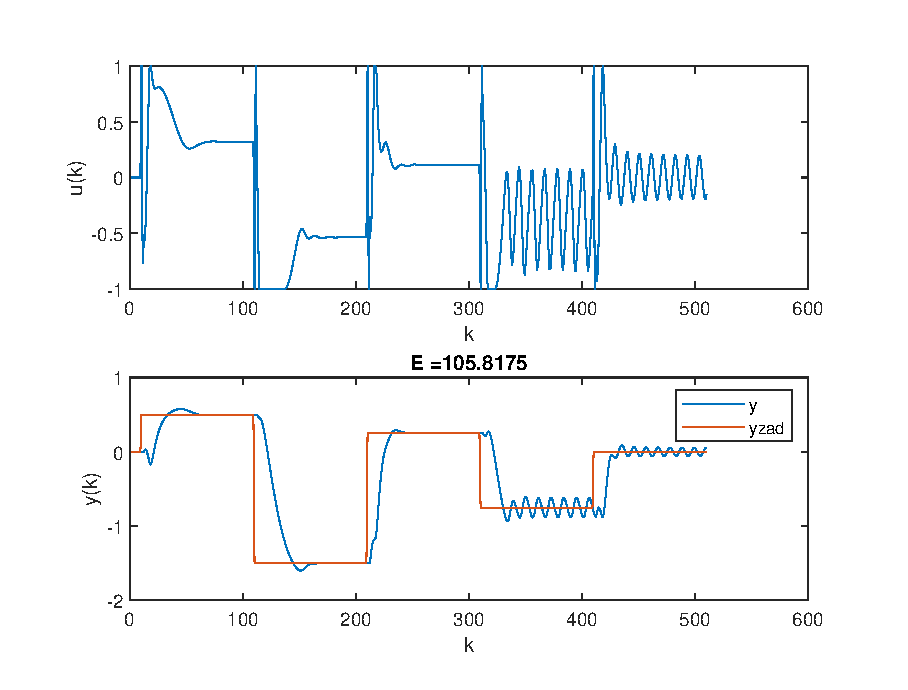
\includegraphics[width=\linewidth]{img/strojeniePID_Ziegler_Nichols.eps}
			\caption{Działanie regulatora PID z nastawami Kp = 2.4, Ti = 6.5, Td = 1.625}
			\label{fig:PID1}
		\end{figure}
		
		\newpage
	\section{NO}
		\label{sec:NO}
		Algorytm NO, tym różni się od algorytmu NPL, że do wyznaczania predykcji wyjścia stosuje się model nieliniowy. Oznacza to, że nie można wyznaczyć przyszłych sterowań analitycznie. Posługując się wskaznikiem jakości
		\begin{equation}
		\begin{tabular}{l}
		$J(k) = \sum\limits_{p=1}^{N}(y^{zad}(k)-\hat{y}(k+p|k))^2+\lambda\sum\limits_{p=0}^{N_u}(\Delta u(k+p|k))^2$
		\end{tabular}
		\label{eq:wsk_jakosc}
		\end{equation}
		wyznacza się takie sterowania dla których jest on najmniejszy.
		Wyliczyjąć predykcje wyjścia jako
		\begin{equation}
		\begin{tabular}{l}
		$\hat{y}(k+p|k)=w20 + w2*tanh(w10+w1*x(k+p|k))+dk$
		\end{tabular}
		\label{eq:NO_wyjscie}
		\end{equation}
		gdzie
		\begin{equation}
		\begin{tabular}{l}
		$x(k+p|k)=\begin{bmatrix}u(k-3+p)\\u(k-4+p)\\y(k-1+p)\\y(k-2+p)\end{bmatrix}$
		\end{tabular}
		\label{eq:NO_wesn}
		\end{equation}
		We wzorze tym, podobnie jak w równaniu \ref{eq:NPL_y0} i \ref{eq:GPC_y0} dla $y(k+p|k)=\hat{y}(k+p|k)$. Dodatkowo, ponieważ przewidujemy jedynie przez cały horyzont sterowania, zakłada się, że sterowanie dla $p>Nu-1$ przyjmuje wartość $u(k+p)=u(k+N_u-1)$. Mając wyznaczone wszystkie wartości można obliczyć zadanie optymalizacji. W tym celu wykorzystaliśmy obecny w Matlabie algorytm $fmincon$, a optymalizowaną przez nas zmienną było Nu przyszłych sterowań licząc z aktualnym.
		Regulator NO był testowany z użyciem sieci neuronowej wytrenowanej algorytmem BFGS z użyciem rekurencji opisanej w sekcji \ref{sec:bfgs}. Wyniki działania algorytmu NO przedstawione są na rysunku \ref{fig:NO}. Jak widać zarówno wyjście obiektu jak i sterowania wyglądają świetnie. Nie występują oscylacje ani przesterowania, a sterowanie jest dosyć łagodne. Niestety dużą wadą algorytmu NO jest, fakt że w każdym kroku algorytmu należy rozwiązać zadanie nieliniowej optymalizacji, co w przypadku obiektów o dłuższych horyzontach predykcji potrafi prowadzić do bardzo długiego czasu wyznaczania sterowań.
		
		\begin{figure}[h!]
			\centering
			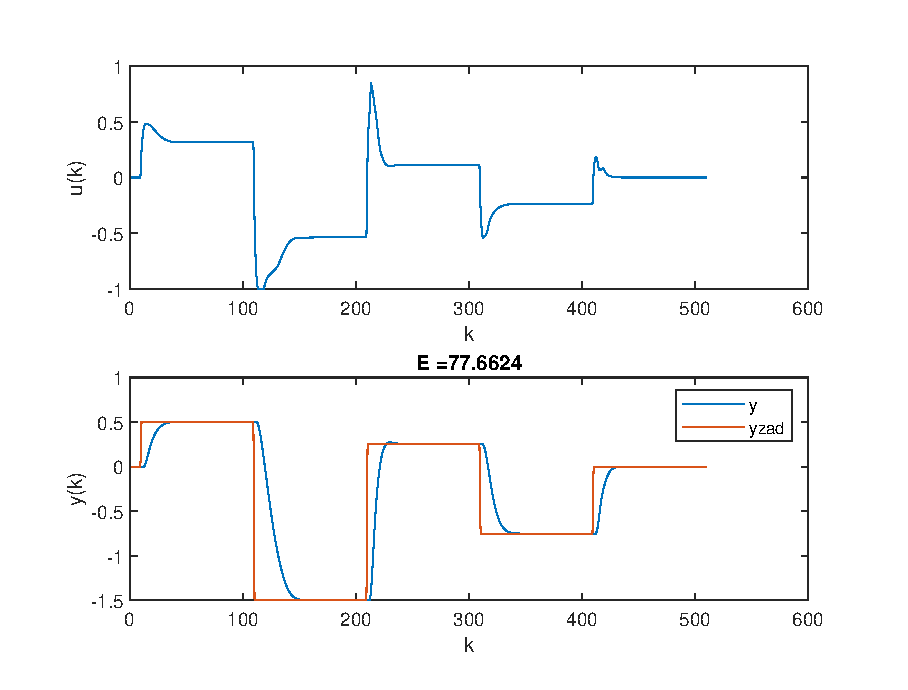
\includegraphics[width=0.7\linewidth]{img/strojenieNO_N_19_Nu_2_lam_4.eps}
			\caption{Działanie regulatora NO z nastawami N=19, Nu=2, $\lambda$=4}
			\label{fig:NO}
		\end{figure}